\documentclass[10pt,a4paper]{report}
\usepackage[utf8]{inputenc}
\usepackage{amsmath}
\usepackage{amsfonts}
\usepackage{amssymb}
\usepackage{graphicx}

\author{Helena Brekalo}
\begin{document}


\begin{titlepage}

\newcommand{\HRule}{\rule{\linewidth}{0.5mm}} % Defines a new command for the horizontal lines, change thickness here

\center % Center everything on the page
 
\textsc{\LARGE KU Leuven}\\[1.5cm] % Name of your university/college
\textsc{\Large Ma Ingenieurswetenschappen: Computerwetenschappen}\\[0.5cm] % Major heading such as course name


\HRule \\[0.4cm]
{ \huge \bfseries Bedrijfskunde $\&$ Entrepreneurship}\\[0.4cm]
\HRule \\[1.5cm]


\textsc{\large Lesnota's}\\[0.5cm] % Minor heading such as course title


\Large \emph{Author:}\\
Helena \textsc{Brekalo}\\[3cm]

{\large 2015-2016}\\[3cm] % Date

\vfill % Fill the rest of the page with whitespace

\end{titlepage}

\tableofcontents
\clearpage

\chapter{Les 1}

\section{Slides: 1\_Bedrijfskunde\_Inleiding(1)}

\paragraph{Slide 6:} $\sim$Productlevencyclus: tijd waarin men nieuwe producten verwacht verkort $\&$ men wil steeds meer persoonlijke dingen (vari\"eteit). Zie Figuur \ref{les1_01}.

\begin{figure}[h!]
\centering
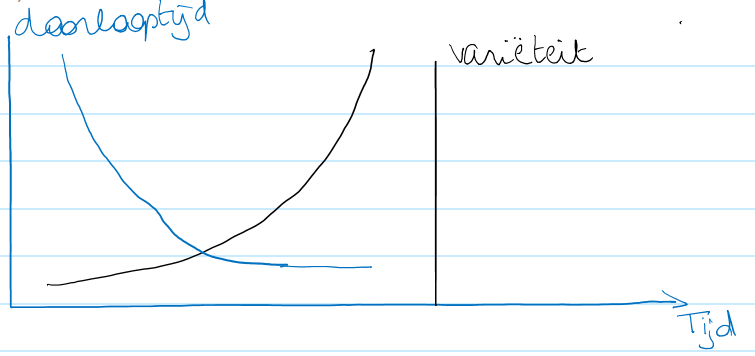
\includegraphics[width=90mm]{Les1_Slide6.png}
\caption{Productlevencyclus} 
\label{les1_01}
\end{figure}

\paragraph{Slide 8:} Bedrijfseconomisch luik: voorspellingstechnieken: je hebt je product en je moet weten hoeveel je de komende maanden en jaren gaat produceren en welke consequenties daaraan hangen.\\
ERP: bv IER en ISP, personeelsbestanden, boekhouding,… 

\paragraph{Slide 10:} Set kleine vraagjes: vooral over begrippen (JIT, MRP,…). Let goed op verwoording en denk goed na over het antwoord! Bv: investering waarbij je 100 000 euro uitgeeft en je krijgt de volgende 5 jaar 30 000 terug, willen we nagaan of het interessant is. Als de waarde van het geld hetzelfde blijft, is het interessant. Kom niet af dat je rekenfouten gemaakt hebt op het examen!

\paragraph{Slide 13 $\&$ 14:}
\begin{itemize}
\item 5000 v.C. daar heeft men een aantal zaken teruggevonden die tonen dat men al bezig was met een soort boekhouding: bijhouden voorraden, leningen, uitgaven,… Daar werden dus al zaken opgevolgd.
\item Egyptische piramides: tonnen stenen moesten aangebracht worden, maar er waren ook enorm veel mensen aan het werken die moesten eten, slapen, verzorgd worden,…
\item 3000v.C.: volledig ontwikkeld staatssysteem.
\item Code van Hammurabi: men sprak al over minimumlonen.
\item Hannibal: logistieke organisatie om met heel die troep over te steken en eten te voorzien.
\item Feodale systemen: hi\"erarchische systemen: keizer met leenheren,… tot aan de lijfeigenen. De keizer kan niet alles voorzien dus gaat die een organisatiestructuur opbouwen die voor hem het best past. Je krijgt dan een baas die een aantal taken delegeert (bv. belastingen heffen, waarvan een deel moet worden afgestaan aan de keizer $\&$ manschappen sturen in tijden van oorlog).
\item 1300: dubbele boekhouding en kostberekeningen.
\item 1436: scheepswerf in Venetië: flowshop (alle producten volgen dezelfde weg: je hebt een aantal stations en men start met een skelet en op het einde heeft men een afgewerkte boot). Dit is zo'n bekend voorbeeld omdat er daar toen 2000 werknemers werkten en die slaagden erin om 100 boten te maken in minder dan 2 maanden. Er was dus een volledige organisatie van de lijn, de toevoer, het eten,…
\item 1700 e.v.: industri\"ele Revolutie: men bouwde stoommachines etc.: massaproductie. Men is gestart met gespecialiseerde taken, bouwmachines en massaproductie. Uitwisselbare stukken: men kan stukken gebruiken in verschillende machines: minder voorraad van die stukken nodig want je kan ze op meerdere plaatsen gebruiken. Bv kopiemachines: worden al voor 3e of 4e keer gebruikt. Zo'n 80\% van een oude machine is nog bruikbaar en wordt dus hergebruikt.
\item 1886: eerste keer ingenieur als economist $\rightarrow$ industrial engineering.
\item Henri Fayol: je moet denken aan productie, veiligheid, sturen plannen, accountancy,… $\rightarrow$ extra zaken die aan bod komen.
	\end{itemize}
	
\paragraph{Slide 15:} Ondernemen: er zijn mensen, materialen,…\\
Schumpeter: gebruikte de term ``ondernemer'' voor het eerst in de vorm van innovator. \\
Bedrijven worden alsmaar complexer $\&$ de klant komt meer centraal te staan: hij wil meer en sneller. Er wordt ook meer gekeken naar duurzame zaken. 

\paragraph{Slide 16:} Massaproductie etc kan problemen geven (realisatie) $\rightarrow$ biedt kortetermijnwinst. Er is dus langetermijnvisie nodig. \\
Henry Ford: als een bedrijf alleen maar winst wil maken, zou het eigenlijk niet mogen bestaan. Er is ook maatschappelijke bijdrage,… nodig. Toen is men de zaken anders beginnen bekijken.\\
Club van Rome: we moeten op een andere manier tewerk gaan om ervoor te zorgen dat we nog een paar 100 jaar kunnen voortgaan.

\paragraph{Slide 17:} Men moet duurzaam werken en men moet proberen voldoen aan de noden van vandaag op zo'n manier dat we de toekomst niet compromiteren.

\paragraph{Slide 19 - 22:} Veel bedrijven willen meewerken aan duurzaamheid. Als je hun jaarverslagen neemt, zie je dat ze daar ook over duurzaamheid praten.

\paragraph{Slide 23:} Een bedrijf staat niet op zichzelf dus je moet kijken naar de positie van de onderneming. Verschillende standpunten: gebruikers (mensen die producten aankopen: hebben bepaalde verwachtingen), de maatschappij (werkgelegenheid gewenst, diensten die iets voor hen doen), verwachtingen van het individu, markten (concurrenten!).\\
Een bedrijf is een economisch maar ook een sociaal systeem: zie \textbf{Slide 24:} aandachtspunten van Lotus op het sociaal systeem.

\paragraph{Slide 25:} Een bedrijf moet een meerwaarde cre\"eren, afkomstig van inkomsten en en uitgaven. Het verschil tussen beide is de meerwaarde. Je gebruikt die meerwaarde om lonen te betalen, belastingen, vergoeding voor het kapitaal, leningen $\&$ autofinanciering (kan gebruikt worden voor investeringen,…).

\paragraph{Slide 26:} Het bedrijf staat tussen leveranciers en klanten. Alle pijltjes zijn dingen die belangrijk zijn, bv levenscyclus: waar bevindt mijn product zich in de markt, wat is zijn levenscyclus?\\ Macht: ben je een grote klant van de leverancier of de enige klant? Dan kun je een aantal zaken doordrukken. Als je maar een kleine leverancier bent, dan zal dat minder zijn.

\paragraph{Slide 30:} Je kan intrapreneurship hebben (binnen een bedrijf) of erbuiten (entrepreneurship). In beide gevallen zoekt men naar innovatie. Schumpeter dacht dat dat vooral kon gevonden worden binnen bedrijven omdat er daar meer geld beschikbaar was. Dat is niet het geval. Naarmate een bedrijf groter wordt, wordt de organisatiestructuur logger en idee\"en die van werknemers komen, komen vaak niet tot ``boven''. In kleine bedrijven komt dat dus meer boven. Mensen die goede idee\"en hebben over aangepaste producten kunnen dat in een box steken in sommige bedrijven en zo gaat men die idee\"en evalueren.

\paragraph{Slide 31:} Een idee moet goed zijn en je moet ervoor zorgen dat de klant dat wil. Normaal moet het zo zijn dat jouw product het probleem van een klant oplost. Het moet een product zijn met duidelijke specificaties en het moet een potenti\"ele markt hebben. Ook rekening houden met concurrentie (bv. wasmachinetablet: vroeger was dat alleen maar in poeder en toen kwam Finish met tabletten en die begonnen 3 maand op voorhand daar reclame voor te maken. 1 week nadat het op de markt was gekomen, kwam een copycat er ook mee op de markt om dus ook een graantje mee te pikken. Het grote voordeel was dat de reclame gemaakt werd door Finish). Je moet voldoende beginkapitaal hebben (zelf hebben, binnenbrengen door investeerders aan te spreken,…). Je moet de juiste mensen aantrekken.

\section{Slides: 2\_Bedrijfskunde\_wat is een bedrijf}

\paragraph{Slide 5:} Er kunnen verschillende standpunten ingenomen worden om te kijken naar bedrijven. 

\paragraph{Slide 6:} De 4 sectoren: 2 laatste samen (tertiaire en kwartaire). De primaire sector neemt zo'n 3\% van BNP in beslag, de secundaire 33\% en de tertiaire en kwartaire de rest. De maatschappij is volledig veranderd van agrarisch naar dienstverlening.

\paragraph{Slide 7:} Je kan het bedrijf in 2 delen splitsen: goederen en diensten. De manier van werken en plannen is hier dikwijls anders. Als je kijkt naar ziekenhuizen, zij leveren ook diensten, dat is nog een stap verder dan hier. Als je naar een bank gaat voor een lening, negoti\"eer je. Als je naar een ziekenhuis gaat voor een operatie, ben je een product want je ondergaat de operatie. 

\paragraph{Slide 11 $\&$ 12:} Aangezien je niet aansprakelijk bent, word je veel meer gecontroleerd op wat je doet. 

\paragraph{Slide 13 e.v.:} Voor welk soort bedrijven.




\end{document}